When describing the Secure CC Protocol, we referred to ``virtual credit cards''.
In this chapter, we describe them more formally.

\section{Virtual Credit Cards}

Many consumer smart phones today support the ability to communicate over NFC.
Indeed, as described in Section \ref{sec:insecure-attacks}, this ability is used by skimmers and relay attackers in order to perform fraudulent purchases.
In a very similar way, this ability can be used by an authorized party to perform non-fraudulent purchases.

A virtual credit card is a device capable of NFC communication, and which emulates a credit card in a CC Protocol.
In its simplest form, it is simply an application running on a smart phone which correctly responds to solicitation messages.
As such, the application must have access to the following information:

\begin{itemize}
\item the credit card number
\item the expiration date
\item the next iCVV
\item the issuing bank name
\end{itemize}

Note that while most of this information is known to the cardholder, the iCVV generation mechanism is not.
In order to be able to generate valid iCVVs, a virtual credit card must have access to the seed from which iCVVs are generated.
As such, a virtual credit card cannot be created without the cooperation of the physical card's issuing bank.


\section{Electronic Wallets}

There is no reason that a smart phone capable of NFC communication should be limited to supporting a single credit card.
Applications such as Google Pay and Apple Wallet exist today,
    allowing a customer uses his smart phone to select the credit card with which to pay for a purchase,
    following which the phone emulates the selected credit card.
We refer to a collection of virtual credit cards and accompanying software
    (e.g. the interface for allowing the customer to select a card, password protection, etc.) as an ``Electronic Wallet'',
    and illustrate its use in Figure \ref{fig:wallet}.

\begin{figure}[h!]
  \caption{Use of an Electronic Wallet}
  \centering
    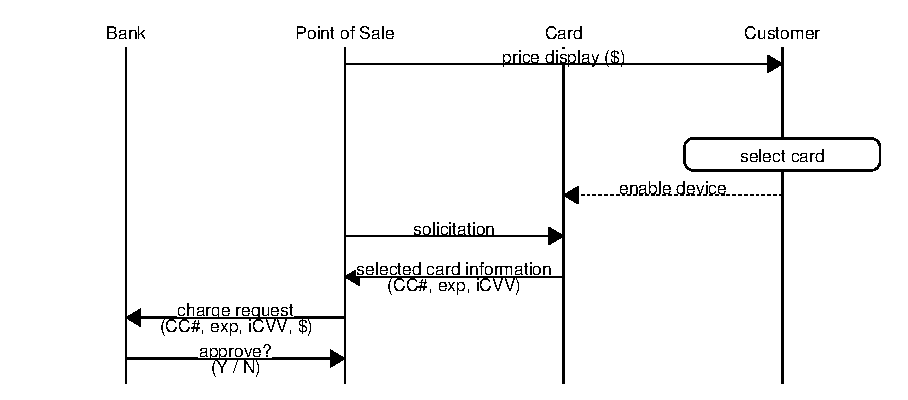
\includegraphics{img/wallet.eps}
  \label{fig:wallet}
\end{figure}

Electronic Wallets are advantageous because for several reasons:
\begin{itemize}
\item Convenience: they allow a customer to carry an essentially unlimited number of credit cards on their person, without taking up extra space
\item Security: they protect the customer from skimming and relay attacks, because they are typically programmed not to respond to solicitations without customer consent
\item Interface: they create a rich interface between the customer and the credit card, enabling the customer to participate in the protocol as in the Secure CC Protocol in Chapter \ref{cha:secure}
\end{itemize}
